\section{Motivation} \label{Motivation}

\begin{displayquote}
  \glqq Weltweit ist die Fleischerzeugung zwischen 2002 und 2012 um 23\% und in Deutschland um 29\% gestiegen. Die globalen Fleischexporte erhöhten sich im gleichen Zeitraum um 60\%, in Deutschland sogar um 124\%. Deutschland zählt sowohl beim Import als auch beim Export von Fleisch- und Fleischprodukten zu den bedeutendsten Handelsnationen weltweit.\grqq{}
\end{displayquote}

\begin{flushright}
  \citet{Efken2015}
\end{flushright}

Lebensmittelsicherheit ist ganz offensichtlich strategisch für die Volksgesundheit und das Wohlbefinden der Gesellschaft. Der öffentliche Druck auf Hersteller für eine ausreichende Kennzeichnung von Produkten und ihre Bestandteile wird stetig größer. Jeder Teil der Lieferkette ist in der Verpflichtung im Falle von Kontamination schnellstmöglich reagieren zu können. \citep{EPER2002}.\\

Vom Rohstofflieferanten bis zum Endkunden gibt es allein in Deutschland ein Netz von Marktteilnehmern mit erheblicher Größe. Knapp 150.000 Betriebe für die Rinder Mast und Milchproduktion, etwa 30.000 Betriebe im Bereich der Schweinehaltung und rund 60.000 Unternehmen für die Geflügelhaltung \citep{Efken2015}. Dabei existiert de facto kein Standard Verfahren zwischen diesen Marktteilnehmern zum Informationsaustausch für die Chargenrückverfolgung. In der Fleischwarenindustrie beispielsweise existieren weit über 140 unterschiedliche Austauschformate zwischen den Teilnehmern einzelner Lieferketten.

Zum jetzigen Zeitpunkt (Stand 2019) findet eine Chargenrückverfolgung daher fast ausschließlich durch einen Datei-Austausch bzw. eine zentrale Datenbank je Teilnehmer der Lieferkette statt. Dabei müssen Informationen für einen mehrstufigen Produktionsporozess bereitgestellt und verarbeitet werden \citep{Siepermann2015}.\\

% \begin{figure}[h!]
% 	\centering
% 	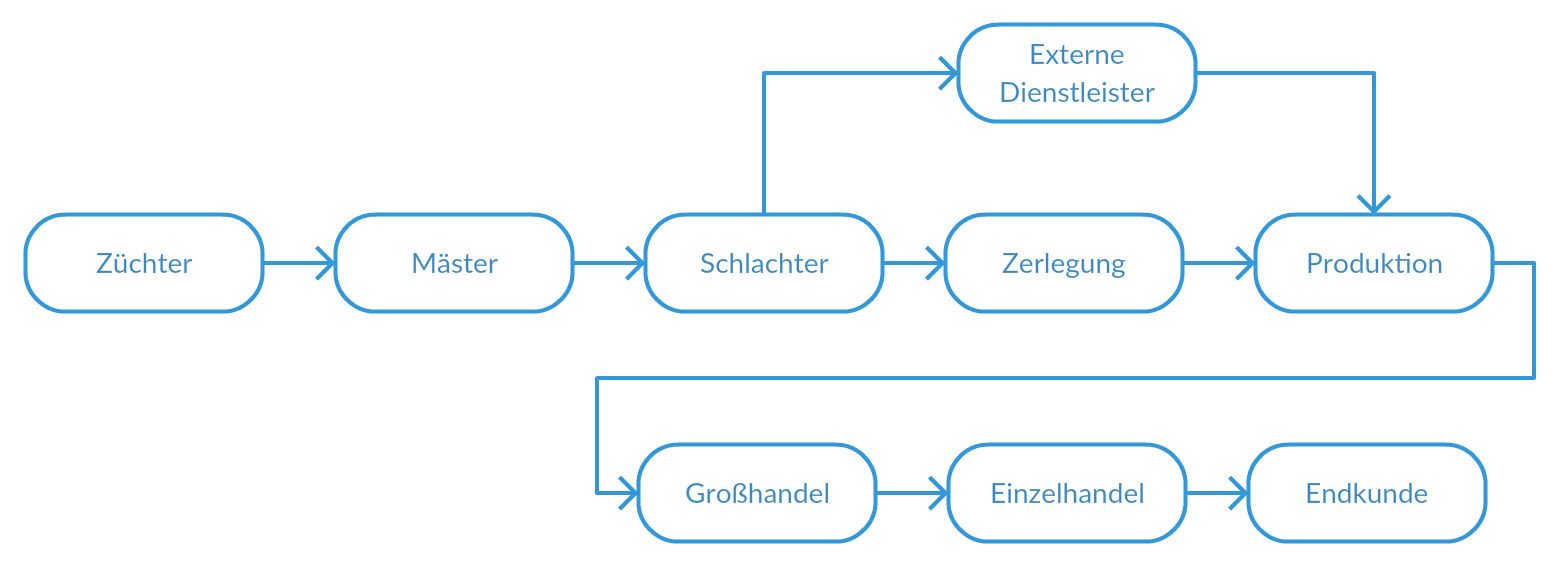
\includegraphics[width=1.0\linewidth]{pictures/Lieferkette-schematisch}
% 	\caption[Schematische Darstellung einer Lieferkette in der Fleischwarenindustrie]{Schematische Darstellung einer Lieferkette in der Fleischwarenindustrie\citep{CIOWSCE2019} (eigene Darstellung)}
% 	\label{fig:lieferkette-schematisch}
% \end{figure}

% Abbildung \ref{fig:lieferkette-schematisch} zeigt schematisch eine Lieferkette innerhalb der Fleischwarenindustrie. Der Abbildung ist zu entnehmen, dass es keine zentrale \glqq Clearing Stelle\grqq{} bzw. Supervisor gibt, welche sämtliche Transaktionen kontrolliert bzw. verifiziert.\\

Aus der geringen Umsatzrendite von -1\% bis +1,5\%  und den dadurch entstehnden Druck am Markt bestehen zu bleiben resultieren immer häufiger Unregelmäßigkeiten innerhalb der Lieferkette. Nur Betriebe in Österreich und Spanien können eine langfristige Rentabilität innerhalb des europäischen Marktes aufweisen \citep{Efken2015}. Ein Beispiel für die genannten Unregelmäßigkeiten ist der Pferdefleisch Skandal aus dem Jahr 2013, bei dem Fleischprodukte nachträglich neu etikettiert und dadurch in Produkten wie Lasagne oder Hamburger Patties weiterverarbeitet wurden \citep{Bundespartei}.\\



\newpage
